\documentclass[12pt]{article}
\usepackage{enumitem}
\usepackage{mathtools}
\usepackage{amsthm}
\usepackage{graphicx}
\graphicspath{ {images/} }
\begin{document}

\title{Assignment 12}
\author{Darwin Ding}
\maketitle

\section*{1. Neural Networks and Backpropagation}
\begin{enumerate}[label=(\alph*)]
	\item 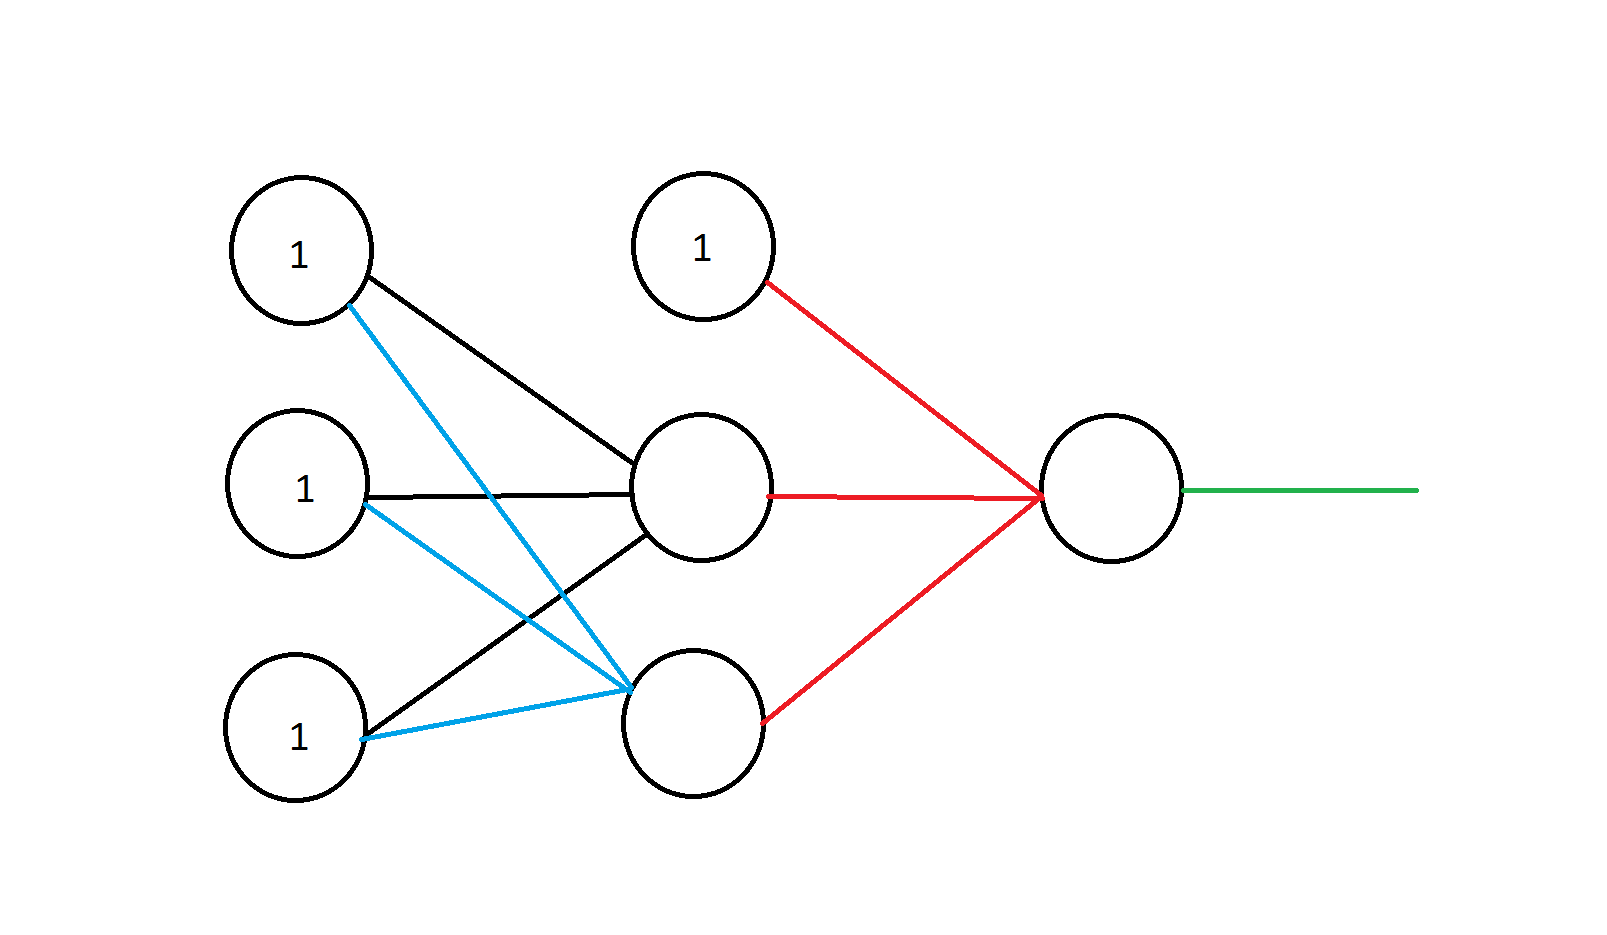
\includegraphics[scale=0.6]{1a.png}
	
	This is a really crude drawing of the neural net for this part. For the sigmoid transformation tanh(x), we end up with $x_0 = [1,1]$, $s_1 = [tanh(.75), tanh(.75)] = [.635148, .635148]$, $x_1 = [1, .635148, .635148]$, $s_2 = [.56757]$, $h(x) = x_2 = \boldsymbol{.5135757}$.
	
	Initializing for back-propagation for tanh, we get $\delta_2 = 2(.5135757 - 1)(1 - .5135757^2) = \boldsymbol{-.71625}$. $\delta_1 = \boldsymbol{[-0.10683, -0.10683]}$
	
	Now we can easily attain the partial derivatives for the final step:
	$\frac{de}{dW_1}$, $\frac{de}{dW_2}$ and thus the final gradient (which is just the set of the partial derivatives) are below. Note that "d1" and "d2" correspond to $\delta_1$ and $\delta_2$ respectively.
	
	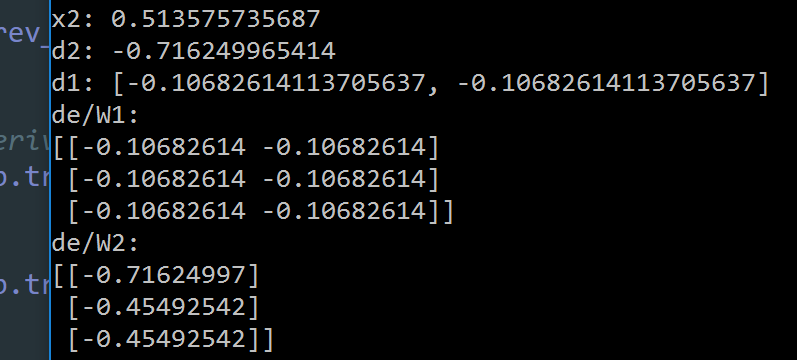
\includegraphics{1a2.png}
	
	Instead of displaying the entirety of the math for the identity as opposed to the tanh function, below are all of the relevant values. Note that, again, the gradient is simply the set of the partial derivatives below.
	
	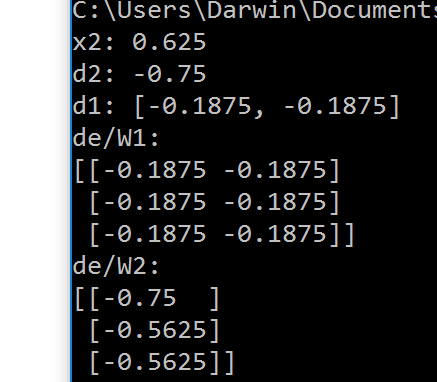
\includegraphics{1a3.png}
	\item Below are the values for the tanh transform neural net with slightly modified weights of $.2501$. There is pretty negligible difference. Again, d1/d2 mean $\delta_1$ and $\delta_2$.
	
	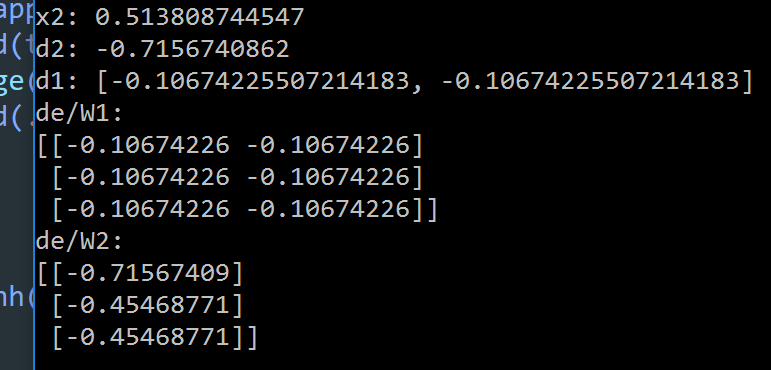
\includegraphics{1a4.png}
	
	Additionally, here are the same weights with the identity transform neural net.
	
	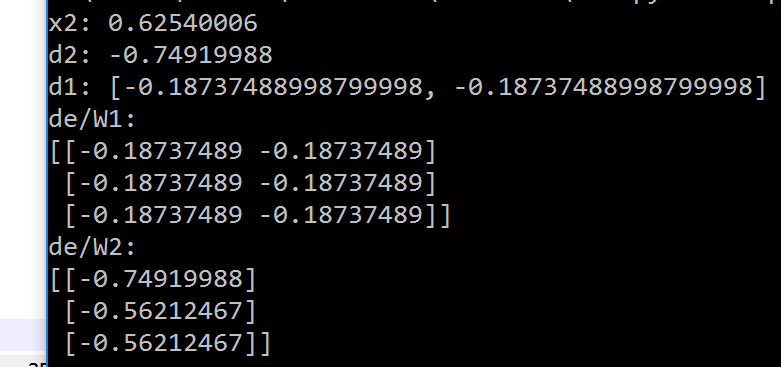
\includegraphics{1a5.png}
\end{enumerate}

\section*{2. Neural Network with Digits}
\begin{enumerate}[label=(\alph*)]
	\item Below is the graph of $E_{in}$ versus iterations. The variable gradient descent was run up to 2 million iterations, but I typically found it converging around 10000.
	
	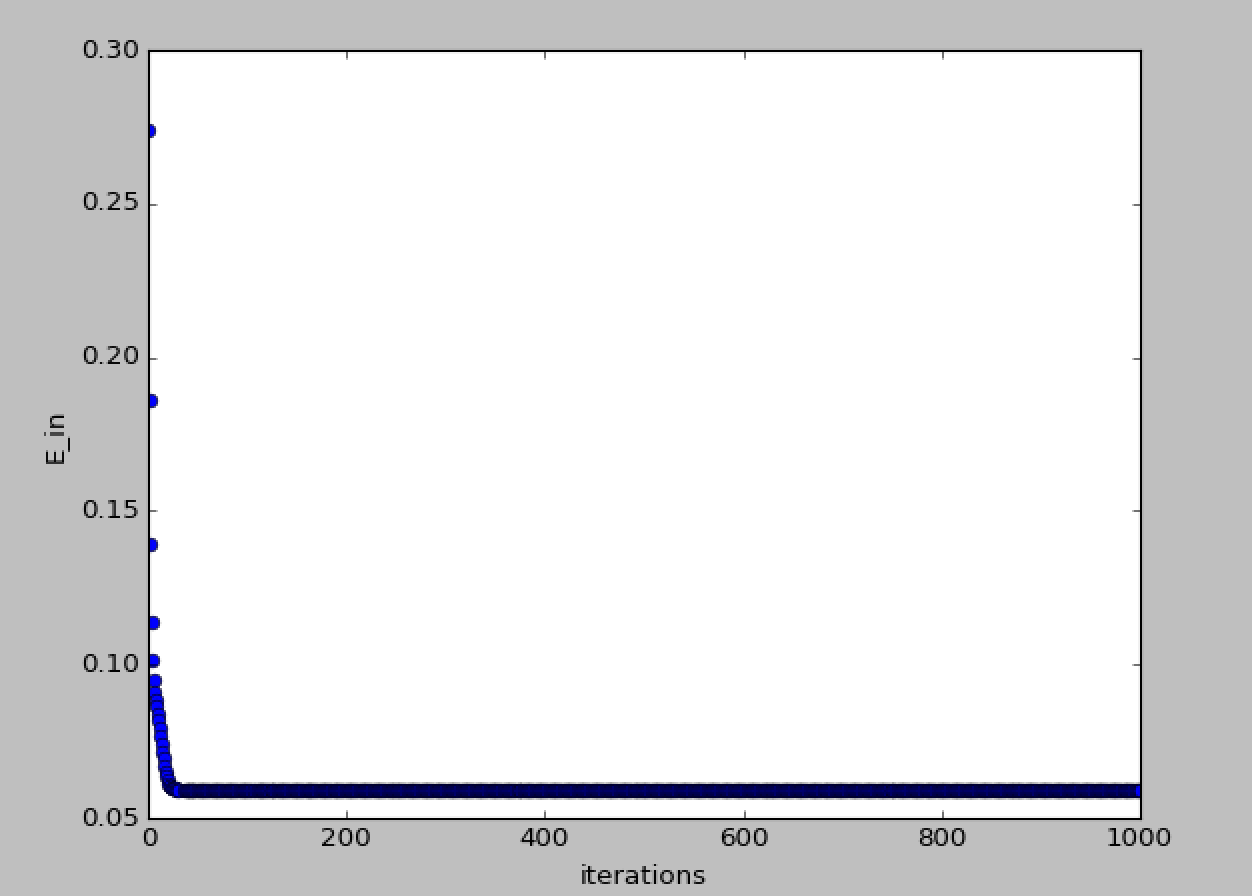
\includegraphics[scale=0.6]{2a1.png}
	
	Additionally, below is the decision boundary. It is doing some classification in a strangely linear fashion, but isn't too shabby. It still has an $E_{in}$ of \textbf{0.0586}.
	
	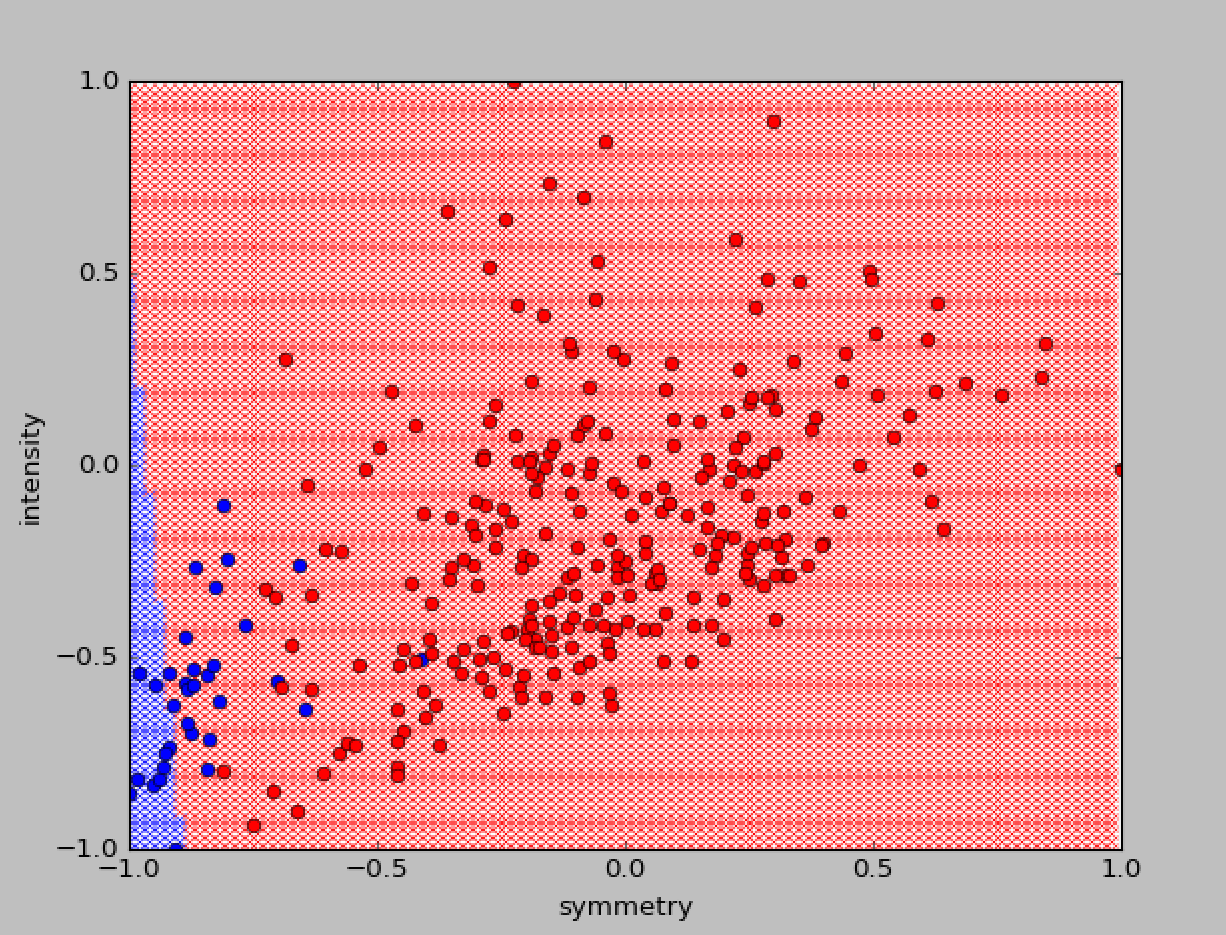
\includegraphics[scale=0.6]{2a2.png}
	
	\item Below is the graph of $E_{in}$ versus iterations for the variable gradient with a weight decay as specified in the problem description. It's hard to see on the graph but this graph converges a little earlier than the other one.
	
	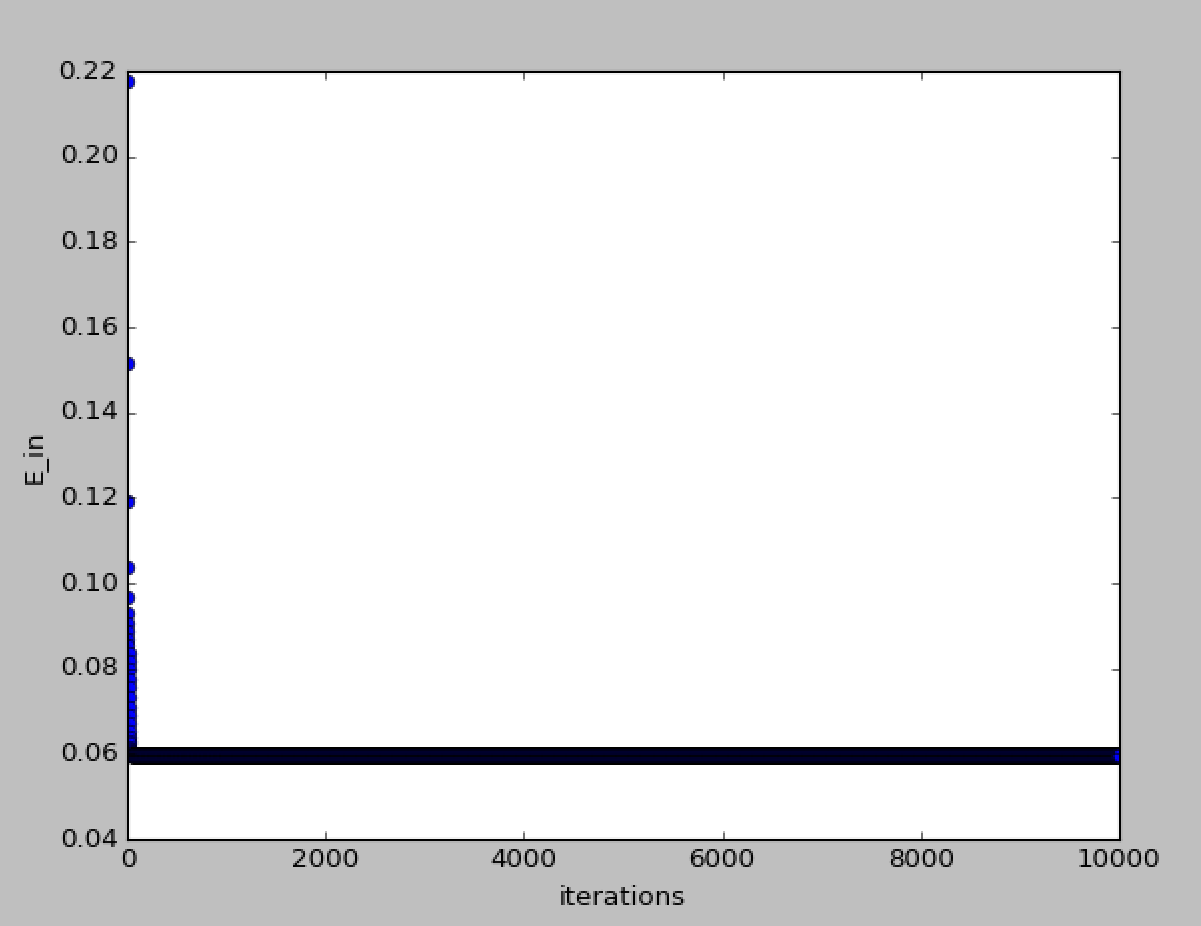
\includegraphics[scale=0.6]{2b1.png}
	
	Additionally, below is the decision boundary. The $E_{in}$ is a little worse now, at \textbf{0.05947}. The classifier has become a little worse, but at least we've made some gain from regularizing.
	
	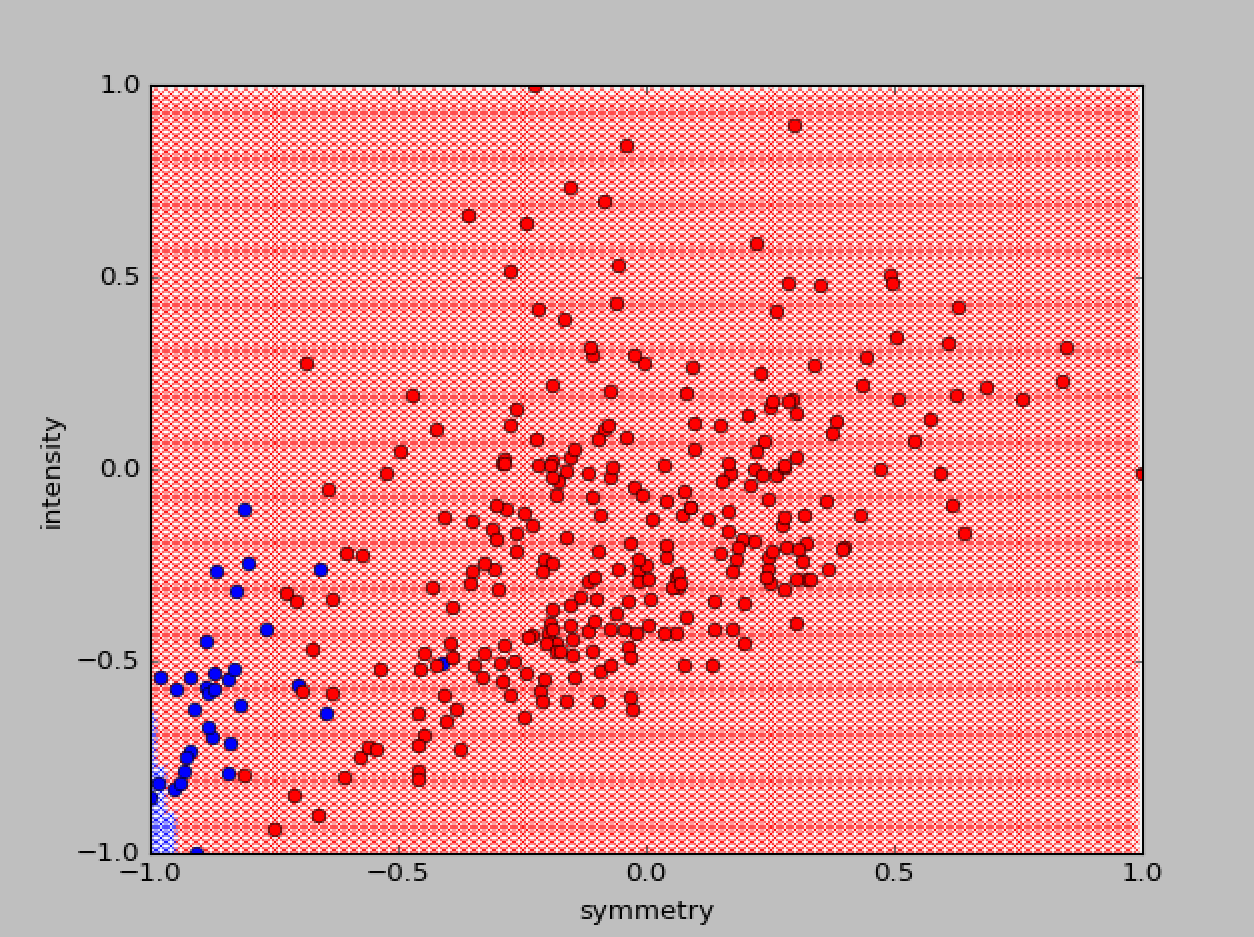
\includegraphics[scale=0.6]{2b2.png}
	
	\item I ran the algorithm with an implemented validation and training set, and found that the validation set error was converging just like the training set. However, it did go up very marginally after a certain point, and had a local minimum at $E_v = \boldsymbol{.055}$.

	Below is a graph of the validation set error (red) and the $E_{in}$ error (blue) over time:
	
	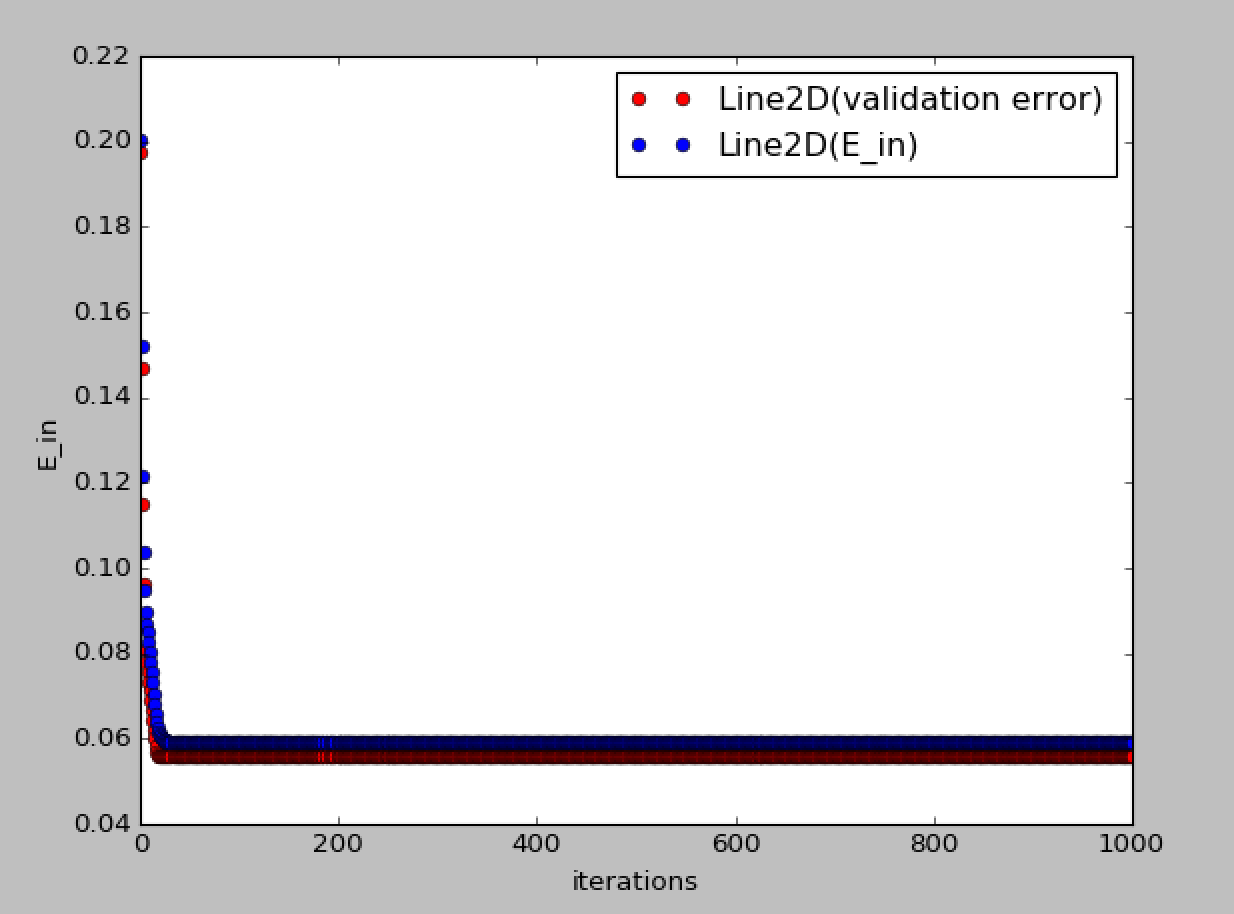
\includegraphics[scale=0.6]{2c1.png}
	
	And then additionally, the final graph using the weights with lowest validation error instead of the actual error, which got me an $E_{in}$ of \textbf{.0592}.
	
	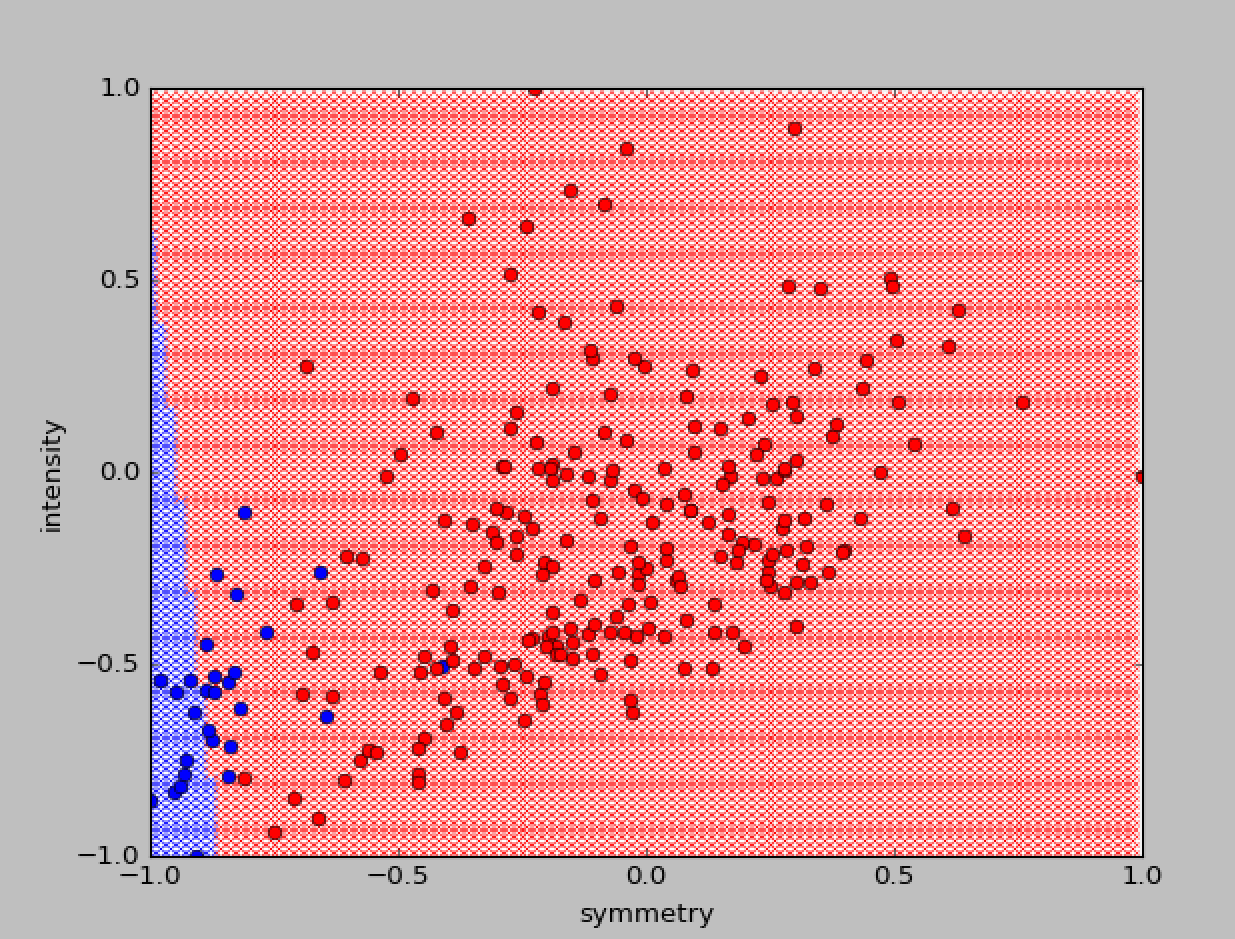
\includegraphics[scale=0.6]{2c2.png}
	
	The error is a very marginally worse using this algorithm because it relies on the validation set error instead of the $E_{in}$ error, but we can trust that it has better generalization error because of the randomly assorted test set.
\end{enumerate}

\section*{3. Support Vector Machines}
\begin{enumerate}[label=(\alph*)]
	\item A hyper-plane in this 2-dimensional space is simply a line, and it is pretty intuitive that the best way to split the two points with the largest cushion is by drawing the line $\boldsymbol{x = 0}$. By moving the line any closer to either point, you cushion the other point harder but lower the overall cushioning by more than you gain.
	\item In this new space, [1, 0] becomes [1, 0] and [-1, 0] becomes [-1, 0]. The points are overall unchanged mostly due to the nature of 1s and 0s with exponents. Again, the optimal hyperplane here will be $\boldsymbol{z_1 = 0}$, but this will not end up being a line in X-space.
	\item Below are the classifiers in X and Z space. The blue line is the $\boldsymbol{x = 0}$ line, and the red line is the $\boldsymbol{z_1 = 0}$ one in Z-space. The two blue points on either side are the actual points in X and Z-space.
	
	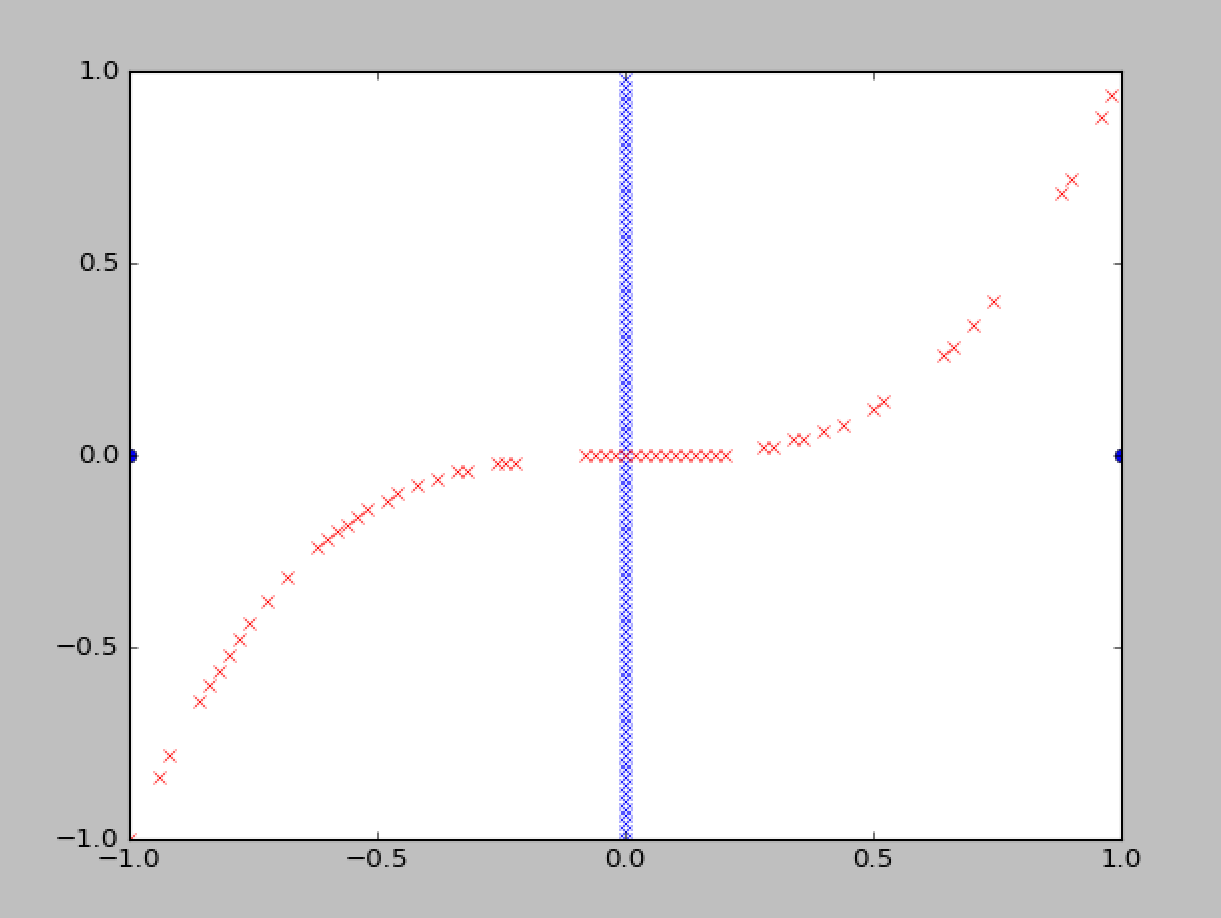
\includegraphics[scale=0.6]{3a.png}
	
	\item After transforming [$x_0$, $x_1$] and [$y_0$, $y_1$], we get [$x_0^3 - x_1$, $x_0x_1$] and [$y_0^3 - y_1$, $y_0y_1$]. The dot product of these two is:
	
	\begin{gather*}
		[(x_0^3 - x_1)(y_0^3 - y_1), x_0x_1y_0y_1]
		\\ = x_0^3y_0^3 - x_0^3y_1 - x_1y_0^3 + x_1y_1 + x_0x_1y_0y_1
	\end{gather*}
	\item The kernel function as a classifier when written in functional form can really be boiled down to $h(x) = sign(x^3 - y)$ for any point (x, y).
\end{enumerate}

\section*{4. SVM with digits data}
\begin{enumerate}[label=(\alph*)]
	\item Below are the decision boundaries for the SVM being run with the 8th polynomial transform with a regularizer $C = 1.0$. It is a pretty solid boundary that has very decent error of \textbf{0.0616}.
	
	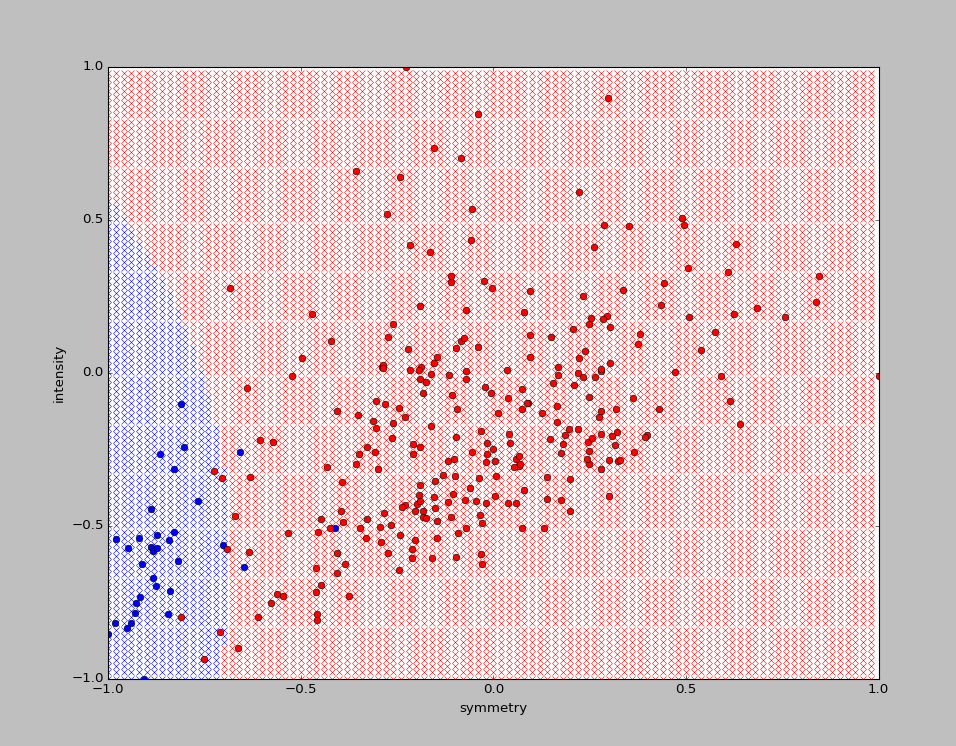
\includegraphics[scale=0.6]{4a1.png}
	
	Additionally, when regularization is bumped up to $C = 100.0$, here are the boundaries. This had a very good $E_{in}$ of \textbf{0.0491}.
	
	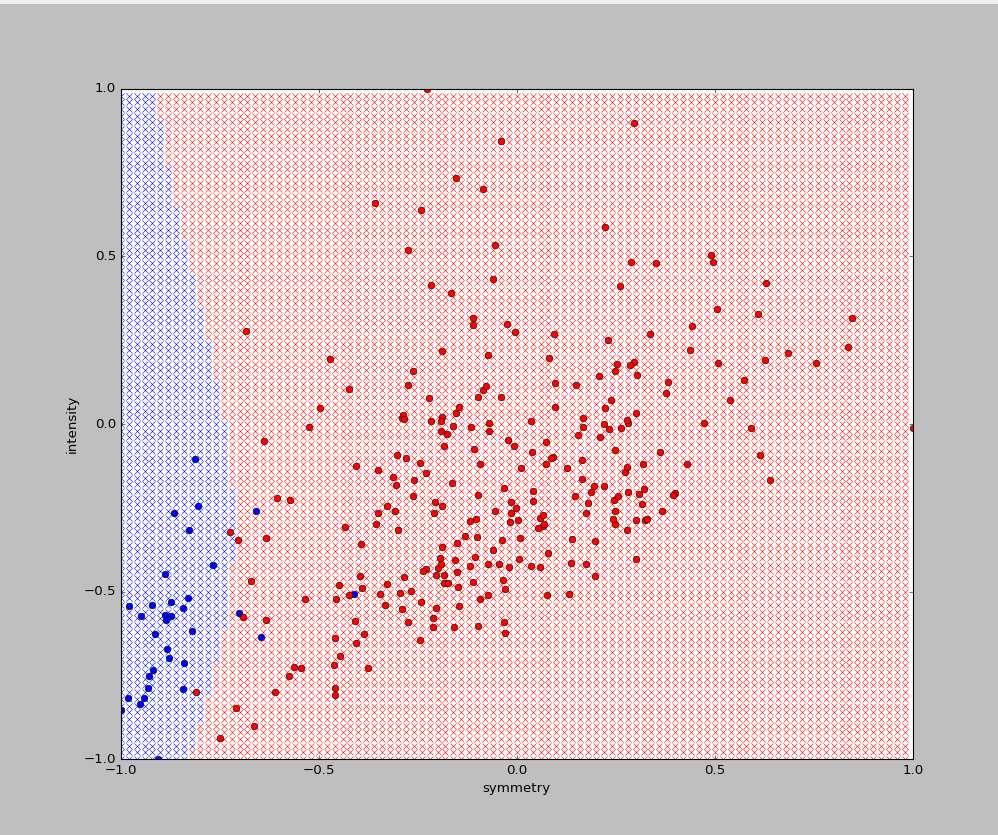
\includegraphics[scale=0.6]{4a2.png}
	
	\item With a higher C, you would expect (as shown above) the boundaries to be more complex. For instance, in the top graph there were quite a few red points in the blue region, but in the bottom graph the high power of the SVM was able to expertly dodge them. This lower $E_{in}$ trades off with generalization power, of course.
	
	\item After iterating over various values between 1.0 and 100.0, I found that the $E_{cv}$ was lowest at $C = 25$ with an $E_{cv}$ of \textbf{0.035} and an $E_{test}$ of \textbf{0.0491}. Below are the decision boundaries for this:
	
	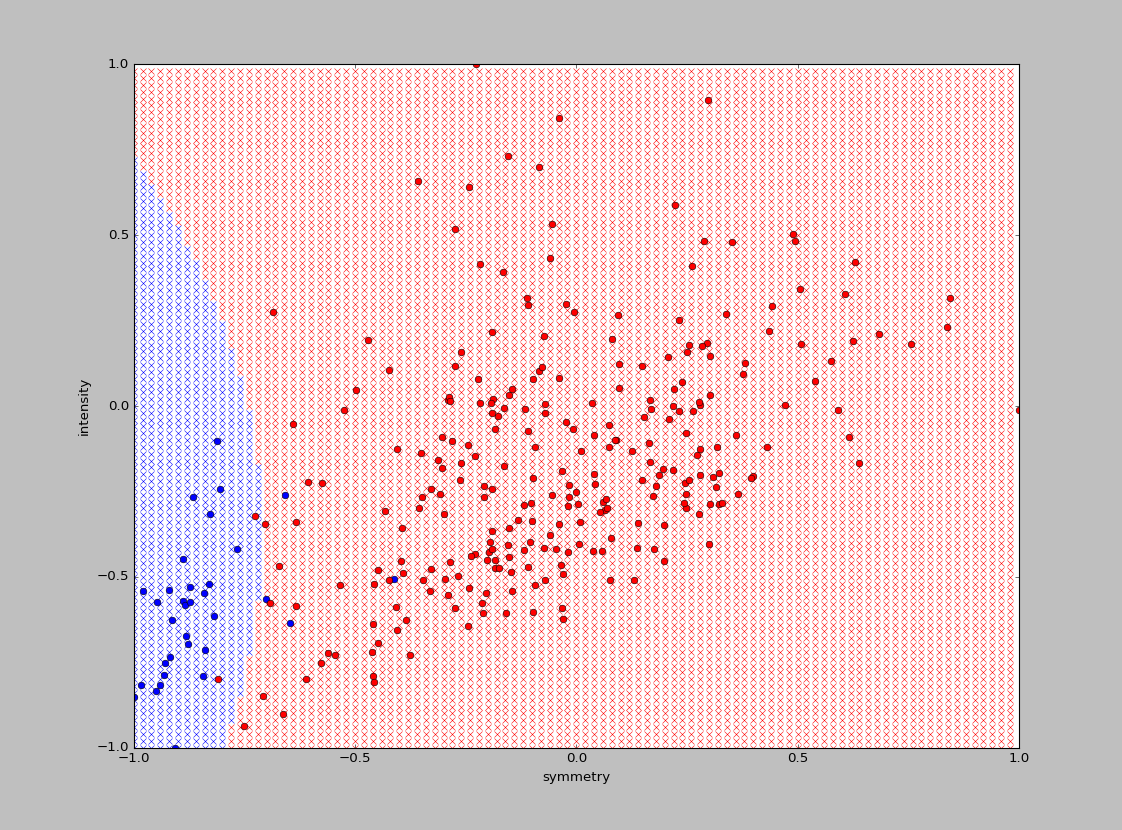
\includegraphics[scale=0.6]{4a3.png}
\end{enumerate}

\section*{5. Compare Methods}
The final test error after applying the straight linear model was $\boldsymbol{.0388}$. The 7-NN rule applied earlier had an $E_{test}$ of $\boldsymbol{0.027}$. The RBF-network returned a test error of $\boldsymbol{0.21}$. The neural net had an $E_{validation}$ of $\boldsymbol{0.055}$. The SVM had an $E_{test}$ of $\boldsymbol{0.0491}$.

I would have the most confidence in the 7-NN rule, because it seems to have the most regularization applied. The linear model has a quite low error but it also uses an 8th polynomial transform. The RBF model had a wildly bad error, but that could've been implementation based. The neural net had decent error, but I suspect that 10 hidden units makes it a little out of control in terms of what it can do after two million iterations. The SVM had decent performance on the test set, but uses an 8th polynomial kernel which is also a little much, but given a small enough C we can try to keep it in check.

Last thing to note is that there is of course data snooping present, because everything has been scaled from -1 to 1 regardless of whether it was in the test or training set.

\end{document}